\subsection{可视化模块}

\par 该模块主要负责窗口管理、实时渲染引擎、数据传输、交互控制以及动画同步,
涉及的类包括\texttt{Gui}(见表\ref{table:Gui})、\texttt{Window}(见表\ref{table:Window})、\texttt{Object}、\texttt{Camera}(见表\ref{table:Camera})和\texttt{GLSpace}(见表\ref{table:GLSpace}),类图和时序图如图\ref{fig:class5}、图\ref{fig:sequence5}所示。

\begin{figure}[htbp]
	\centering
	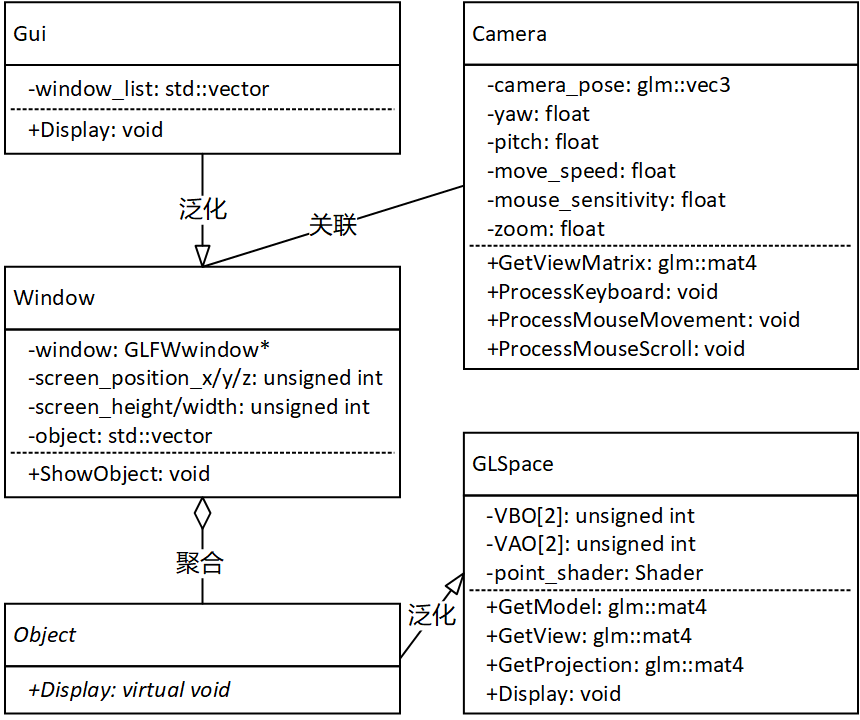
\includegraphics[width=0.7\textwidth]{figures/uml/class5.png}
	\caption{可视化模块类图}
	\label{fig:class5}
\end{figure}

\begin{table}[htbp]
	\centering
	\caption{Gui类的主要成员和方法}
	\label{table:Gui}
	\begin{tabular}{|l|m{3cm}|m{5cm}|m{4cm}|}
		\hline
		   & \multicolumn{1}{c|}{名称}                & \multicolumn{1}{c|}{类型}                                                   & \multicolumn{1}{c|}{功能}        \\
		\hline
		成员 & \centering\arraybackslash window\_list & \centering\arraybackslash vector\textless{}GLFWwindow*\textgreater{} & \centering\arraybackslash 窗口队列 \\
		\hline
		方法 & \centering\arraybackslash  Display     & \centering\arraybackslash void                                            & \centering\arraybackslash 展示窗口 \\
		\hline
	\end{tabular}
\end{table}

\begin{table}[htbp]
	\centering
	\caption{Window类的主要成员和方法}
	\label{table:Window}
	\begin{tabular}{|l|m{3cm}|m{4cm}|m{5cm}|}
		\hline
		                    & \multicolumn{1}{c|}{名称}                       & \multicolumn{1}{c|}{类型}                                               & \multicolumn{1}{c|}{功能}                           \\ \hline
		\multirow{6}{*}{成员} & \centering\arraybackslash window              & \centering\arraybackslash GLFWwindow                                  & \centering\arraybackslash 动画窗口                    \\ \cline{2-4}
		                    & \centering\arraybackslash screen\_position\_x & \centering\arraybackslash unsigned int                                & \centering\arraybackslash \multirow{2}{*}{窗口中心坐标} \\ \cline{2-3}
		                    & \centering\arraybackslash screen\_position\_y & \centering\arraybackslash unsigned int                                &                                                   \\ \cline{2-4}
		                    & \centering\arraybackslash screen\_width       & \centering\arraybackslash unsigned int                                & \centering\arraybackslash \multirow{2}{*}{窗口尺寸}   \\ \cline{2-3}
		                    & \centering\arraybackslash screen\_height      & \centering\arraybackslash unsigned int                                &                                                   \\ \cline{2-4}
		                    & \centering\arraybackslash object              & \centering\arraybackslash vector\textless{}Object*\textgreater{} & \centering\arraybackslash 需要可视化的物体                \\ \hline
		\multirow{1}{*}{方法} & \centering\arraybackslash ShowObject          & \centering\arraybackslash void                                        & \centering\arraybackslash 对物体进行可视化                \\ \hline
	\end{tabular}
\end{table}

\begin{table}[htbp]
	\centering
	\caption{GLSpace类的主要成员和方法}
	\label{table:GLSpace}
	\begin{tabular}{|l|m{3cm}|m{4cm}|m{5cm}|}
		\hline
		                    & \multicolumn{1}{c|}{名称}                 & \multicolumn{1}{c|}{类型}                & \multicolumn{1}{c|}{功能}          \\ \hline
		\multirow{3}{*}{成员} & \centering\arraybackslash VBO{[}2{]}    & \centering\arraybackslash unsigned int & \centering\arraybackslash 顶点缓冲对象 \\ \cline{2-4}
		                    & \centering\arraybackslash VAO{[}2{]}    & \centering\arraybackslash unsigned int & \centering\arraybackslash 顶点数组对象 \\ \cline{2-4}
		                    & \centering\arraybackslash point\_shader & \centering\arraybackslash Shader       & \centering\arraybackslash 着色器    \\ \hline
		\multirow{4}{*}{方法} & \centering\arraybackslash GetModel      & \centering\arraybackslash glm::mat4    & \centering\arraybackslash 计算模型矩阵 \\ \cline{2-4}
		                    & \centering\arraybackslash GetView       & \centering\arraybackslash glm::mat4    & \centering\arraybackslash 计算视图矩阵 \\ \cline{2-4}
		                    & \centering\arraybackslash GetProjection & \centering\arraybackslash glm::mat4    & \centering\arraybackslash 计算投影矩阵 \\ \cline{2-4}
		                    & \centering\arraybackslash Display       & \centering\arraybackslash void         & \centering\arraybackslash 绘制动画   \\ \hline
	\end{tabular}
\end{table}

\begin{table}[htb]
	\centering
	\caption{Camera类的主要成员和方法}
	\label{table:Camera}
	\begin{tabular}{|l|m{4cm}|m{3cm}|m{5cm}|}
		\hline
		                     & \multicolumn{1}{c|}{名称}                        & \multicolumn{1}{c|}{类型}             & \multicolumn{1}{c|}{功能}                         \\ \hline
		\multirow{10}{*}{成员} & \centering\arraybackslash position             & \centering\arraybackslash glm::vec3 & \centering\arraybackslash \multirow{5}{*}{相机位姿} \\ \cline{2-3}
		                     & \centering\arraybackslash front                & \centering\arraybackslash glm::vec3 &                                                 \\ \cline{2-3}
		                     & \centering\arraybackslash up                   & \centering\arraybackslash glm::vec3 &                                                 \\ \cline{2-3}
		                     & \centering\arraybackslash right                & \centering\arraybackslash glm::vec3 &                                                 \\ \cline{2-3}
		                     & \centering\arraybackslash world\_up            & \centering\arraybackslash glm::vec3 &                                                 \\ \cline{2-4}
		                     & \centering\arraybackslash yaw                  & \centering\arraybackslash float     & \centering\arraybackslash 偏航角                   \\ \cline{2-4}
		                     & \centering\arraybackslash pitch                & \centering\arraybackslash float     & \centering\arraybackslash 俯仰角                   \\ \cline{2-4}
		                     & \centering\arraybackslash move\_speed          & \centering\arraybackslash float     & \centering\arraybackslash 相机移动速度                \\ \cline{2-4}
		                     & \centering\arraybackslash mouse\_sensitivity   & \centering\arraybackslash float     & \centering\arraybackslash 鼠标敏感度                 \\ \cline{2-4}
		                     & \centering\arraybackslash zoom                 & \centering\arraybackslash float     & \centering\arraybackslash 缩放级别                  \\ \hline
		\multirow{4}{*}{方法}  & \centering\arraybackslash GetViewMatrix        & \centering\arraybackslash glm::mat4 & \centering\arraybackslash 获取视图矩阵                \\ \cline{2-4}
		                     & \centering\arraybackslash ProcessKeyboard      & \centering\arraybackslash void      & \centering\arraybackslash 处理键盘输入                \\ \cline{2-4}
		                     & \centering\arraybackslash ProcessMouseMovement & \centering\arraybackslash void      & \centering\arraybackslash 处理鼠标移动                \\ \cline{2-4}
		                     & \centering\arraybackslash ProcessMouseScroll   & \centering\arraybackslash void      & \centering\arraybackslash 处理鼠标滚轮                \\ \hline
	\end{tabular}
\end{table}

\par 系统的可视化模块由\texttt{Gui}类管理,\texttt{Gui}类负责管理所有的\texttt{Window}实例化对象。每个\texttt{Window}对象代表一个
独立的动画窗口,每个窗口内展示的对象都是\texttt{Object}类或其子类的实例。在这个系统中,\texttt{Window}类将
实例化两个对象,分别命名为\texttt{rgb\_win}和\texttt{semantic\_win},分别对应用于展示RGB信息和语义信息的
动画窗口。每个\texttt{Window}对象都有一个指向全局相机\texttt{Camera}的指针,这个全局相机模拟OpenGL窗口的相机,
将三维空间通过模型-视图-投影(Model-View-Projection,MVP)矩阵变换转换成二维空间,以便在屏幕上显示。
\texttt{Camera}实例化了一系列控制相机视角和位置的参数,以及一系列处理输入和移动的函数。使用统一的全局相机,可以实现RGB动画和语义动画的实时同步。

\begin{figure}[htb]
	\centering
	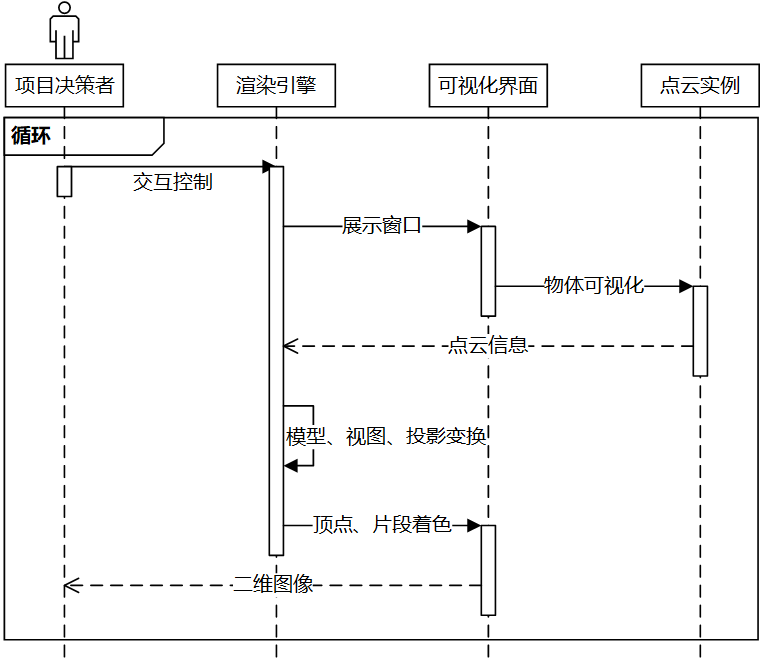
\includegraphics[width=0.7\textwidth]{figures/uml/sequence5.png}
	\caption{可视化模块时序图}
	\label{fig:sequence5}
\end{figure}

\par 为了在窗口中展示点云模型,系统实现了\texttt{GLSpace}类。这个类双继承自\texttt{Object}类和\texttt{Space}类。
\texttt{GLSpace}类实现了\texttt{Display}函数,用于绘制动画,包括点云模型和相机位姿,伪代码算法\ref{algo:Display}所示。同时,它还实现了一系列
计算矩阵的函数,这些函数负责计算模型、视图和投影矩阵。\texttt{GLSpace}类只实例化一个对象,负责在窗口中展示\texttt{Space}对象的点云模型。

\begin{algorithm}[htbp]
	\SetAlgoLined
	\KwData{动画窗口 window}
	\KwResult{点云动画}
	$\textit{点云着色器 point\_shader} \gets \text{顶点着色器 vertex\_shader,片元着色器 fragment\_shader}$\;
	$\text{初始化VBO, VAO}$\;
	$\text{初始化 current\_point\_num 为 0}$\;
	$\text{绑定VAO和VBO}$\;
	\tcp{设置点云的坐标}
	$\text{glVertexAttribPointer}(0, 3, GL\_FLOAT, 0, 6 * \text{sizeof(float)}, (void *)0)$\;
	\tcp{设置点云的颜色}
	$\text{glVertexAttribPointer}(1, 3, GL\_FLOAT, 0, 6 * \text{sizeof(float)}, (void *)(3 * sizeof(float)))$\;
	\While{\text{not} glfwWindowShouldClose(window)}{
		\If{当前窗口 == rgb\_win}{
			$\text{根据两帧间的时间差获取当前帧}$\;
			$\text{计算deltaTime并更新lastFrame}$\;
		}
		$\text{处理窗口的键盘输入}$\;
		$\text{清除颜色和深度缓冲}$\;
		$\text{设置点大小并绘制点}$\;
		\tcp{更新摄像机位置,实质上为每个点计算MVP矩阵}
		$\text{计算MVP矩阵}$\;
		$\text{在 point\_shader 中设置MVP矩阵}$\;
		$\text{设置点大小并绘制点}$\;
		\If{gl\_data\_mtx 未上锁}{
			\If{轮到当前窗口从点云数组中读取数据}{
				$\text{更新 current\_point\_num}$\;
				$\text{为当前窗口加载数据到缓冲对象中}$\;
			}
			$\text{解锁 gl\_data\_mtx}$\;
		}
		$\text{交换前后缓冲}$\;
		$\text{获取并处理事件}$\;
	}
	$\text{删除VAO和VBO}$\;
	\caption{Display}
	\label{algo:Display}
\end{algorithm}

\par 在可视化模块开始运行时,\texttt{Gui}类首先会初始化一个\texttt{Window}对象列表,这个列表存储了所有需要
展示的窗口。接着,通过\texttt{Display}逐个调用列表中每个\texttt{Window}对象的\texttt{ShowObject}函数,展示每个窗
口中的\texttt{Object}对象。这里的\texttt{Object}包括\texttt{GLSpace}类的实例,以及展示相机朝向的向量。

\par \texttt{GLSpace}类同样包含\texttt{Display},负责在\texttt{OpenGL}窗口中绘制出实例化对象。\texttt{Display}首先使用\texttt{VBO}和
\texttt{VAO}在GPU中创建缓冲区,然后使用\texttt{Shader}类加载顶点着色器和片段着色器,最后通过\texttt{GetProjection}、
\texttt{GetView}和\texttt{GetModel}函数计算出MVP矩阵,将三维空间的点云模型投影到二维屏幕上。

\par 为了保证渲染的实时性,数据传输模块会使用双缓冲技术,将点云生成与语义融合模块生成的新
数据传输到OpenGL的缓冲区中,同时,已经在屏幕上显示的旧数据会被保留在另一个缓冲区中,这样可
以防止新旧数据之间的冲突,同时提高渲染的效率。

\par 为了实现交互控制,用户可以通过键盘和鼠标输入,调整相机的位置和视角。\texttt{Camera}的
\texttt{ProcessKeyboard}、\texttt{ProcessMouseMovement}和\texttt{ProcessMouseScroll}函数会根据用户输入的方向、
位移和滚动量,动态调整相机的参数,从而改变相机的位姿和视角。

\par 为了提高可视化的性能,系统可以采用多线程技术并行处理数据,创建两个子线程分别展示RGB动画窗口和语义动画窗口。后续还可以使用GPU加速渲染,通过使用NVIDIA官方提供的\href{https://docs.nvidia.com/cuda/cuda-runtime-api/group__CUDART__OPENGL.html#group__CUDART__OPENGL}{OpenGL Interoperability 系列 API},可以提高系统的渲染效率,提升用户体验。